\documentclass[aspectratio=54,xcolor=dvipsnames]{beamer}
\usetheme{SimpleDarkBlue}

% Packages
\usepackage[utf8]{inputenc}
\usepackage{amsmath, amssymb}
\usepackage{graphicx}
\usepackage{hyperref}
\usepackage{physics}
\usepackage{dsfont}
\usepackage{verbatim}
\usepackage{listings}

\lstset{
    language=Octave,
    basicstyle=\ttfamily\tiny,
    numbers=left,
    numberstyle=\tiny\color{gray},
    stepnumber=1,
    numbersep=8pt,
    backgroundcolor=\color{gray!10},
    showspaces=false,
    showstringspaces=false,
    showtabs=false,
    frame=single,
    rulecolor=\color{gray!70},
    keywordstyle=\color{NavyBlue}\bfseries,
    commentstyle=\color{OliveGreen}\itshape,
    stringstyle=\color{BrickRed},
    breaklines=true,
    breakatwhitespace=true,
    tabsize=4,
    captionpos=b
}


% Title Information
\title{Computational Electromagnetics Project}
\author{Francesco Fischetti}
\institute{Politecnico di Milano}
\date{\today}

\begin{document}

% Title Slide
\begin{frame}
    \titlepage
\end{frame}

% Outline Slide
\begin{frame}{Outline}
    \tableofcontents
\end{frame}


\section{Recall: Maxwell's Equations}
\begin{frame}{Recall: Maxwell's Equations}
    Maxwell's equations in differential form are given by:
    \begin{align*}
        \nabla \cdot \vec{D} &= \rho \\
        \nabla \cdot \vec{B} &= 0 \\
        \nabla \times \vec{E} &= -\frac{\partial \vec{B}}{\partial t} \\
        \nabla \times \vec{H} &= \vec{J} + \frac{\partial \vec{D}}{\partial t}
    \end{align*}

    \begin{center}
    %\scriptsize
    \begin{tabular}{|c|l|c|}
        \hline
        Symbol & Quantity & Unit \\
        \hline
        $\vec{D}(\vec{r})$ & Electric flux density & $C/m^2$ \\
        $\vec{B}(\vec{r})$ & Magnetic flux density & $T$ \\
        $\vec{E}(\vec{r})$ & Electric field & $V/m$ \\
        $\vec{H}(\vec{r})$ & Magnetic field & $A/m$ \\
        $\vec{J}(\vec{r})$ & Current density & $A/m^2$ \\
        $\rho(\vec{r})$ & Volume charge density & $C/m^3$ \\
        \hline
    \end{tabular}
    %\normalsize
    \end{center}
\end{frame}

\begin{frame}{Recall: Constitutive Relations}
    For a linear and isotropic medium the constitutive relations read
    \begin{align*}
        \vec{D} &= \epsilon \vec{E} \\
        \vec{B} &= \mu \vec{H} \\
        \vec{J} &= \sigma \vec{E}
    \end{align*}
    \vspace{0.5em}
    where
    \begin{center}
    \begin{tabular}{|c|l|c|}
        \hline
        Symbol & Quantity & Unit \\
        \hline
        $\epsilon$ & Dielectric permittivity & $[F/m]$ \\
        $\mu$ & Magnetic permeability & $[H/m]$ \\
        $\sigma$ & Electric conductivity & $[S/m]$ \\
        \hline
    \end{tabular}
    \end{center}
\end{frame}

\section{Problem description and Electromagnetic Field Equations}
\begin{frame}{Problem description}
    Consider 2 infinitely long parallel conductors, with cross sections $\Omega_c$, with $c=1,2$. Each conductor is assumed to have electrical conductivity $\sigma_c$, permittivity $\varepsilon_c$, and magnetic permeability $\mu_c$. The electromagnetic problem becomes two-dimensional with translational symmetry. We assume that the conductors are infinitely long in the $z$-direction.
        \begin{figure}[h]
            \centering
            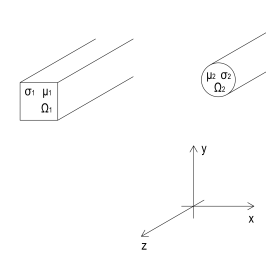
\includegraphics[width=0.35\textwidth]{Images/Conductors_figure.png}
            \caption{Geometry of the two parallel conductors.}
            \label{fig:conductors}
        \end{figure}
\end{frame}

\begin{frame}{The Electromagnetic Field Equations I}
    In multipath eddy current problems where charges and displacement currents are negligible, the steady state time harmonic electromagnetic field is governed by:
    \begin{align}
        \nabla \cdot \tilde{\vec{D}} &= 0 \label{eq:divD} \\
        \nabla \cdot \tilde{\vec{B}} &= 0 \label{eq:divB} \\
        \nabla \times \tilde{\vec{E}} &= - j \omega \tilde{\vec{B}} \label{eq:curlE} \\
        \nabla \times \tilde{\vec{H}} &= \tilde{\vec{J}} \label{eq:curlH}
    \end{align}
    where $j$ is the imaginary unit and $\omega$ is the angular frequency. For the above complex fields, the time dependence is obtained by the substitution:
    \begin{equation*}
        \vec{V}(\vec{r}, t) = \sqrt{2} \cdot \Re \left\{ \tilde{\vec{V}}(\vec{r}) \cdot e^{j \omega t} \right\}
    \end{equation*}
    From now on, we will omit the tilde notation for the complex fields.
\end{frame}

\begin{frame}{The Electromagnetic Field Equations II}
    We introduce the Magnetic Vector Potential (MVP) as
    \begin{equation}
        \vec{B} = \mu \vec{H} = \nabla \times \vec{A}, \qquad \text{ with } \nabla \cdot \vec{A} = 0 \label{eq:divA}
    \end{equation}
    In this case all the variables are constant along $z$ (Figure~\ref{fig:conductors}), and:
    \begin{equation}
        \vec{H} = H_x \vec{e}_x + H_y \vec{e}_y, \qquad
        \vec{J} = J \vec{e}_z, \qquad
        \vec{A} = A \vec{e}_z. \label{ed:2D}
    \end{equation}
    Substituting \eqref{eq:divA} into the Maxwell's equations, we obtain that \eqref{eq:divB} is automatically satisfied, and \eqref{eq:curlH} becomes:
    \begin{equation}
        \nabla \times \left( \frac{1}{\mu} \nabla \times \vec{A} \right) = \vec{J}\label{eq:curlA}
    \end{equation}
    Using \eqref{ed:2D}, we can rewrite \eqref{eq:curlA} as:
    \begin{equation}
        \nabla \cdot \left( \frac{1}{\mu} \nabla A \right) = -J \label{eq:laplacianA}
    \end{equation}
\end{frame}

\begin{frame}{The Electromagnetic Field Equations III}
    The relationship between the electric field $\vec{E}$ and the magnetic vector potential $\vec{A}$ is obtained by substituting equation~\eqref{eq:divA} into equation~\eqref{eq:curlE} and integrating. The result is:
    \begin{equation}
        \vec{E} = -j\omega \vec{A} - \nabla \phi \label{eq:E}
    \end{equation}
    where $\phi$ is the electric scalar potential.
    \newline
    We define:
    \begin{equation}
        \vec{J}_s = - \sigma \nabla \phi, \qquad
        \vec{J}_e = - j \omega \sigma \vec{A},  \qquad 
        \text{so that: } \vec{J} = \vec{J}_e + \vec{J}_s \label{eq:JsJe}
    \end{equation}
    We can also define:
    \begin{equation}
        \vec{A}_s =  \frac{\vec{J}_s}{- j \omega \sigma}
    \end{equation}
    Writing equation~\eqref{eq:JsJe} in scalar form, we have: 
    \begin{equation}
        J = J_e + J_s = - j \omega \sigma A - \sigma \nabla \phi \cdot \vec{e}_z \label{eq:JsJe_scalar}
    \end{equation}
\end{frame}

\begin{frame}{The Electromagnetic Field Equations IV}
    \begin{block}{The System of Equations}
    Combining equations~\eqref{eq:laplacianA} and~\eqref{eq:JsJe_scalar}, we obtain the following system of equations:
    \begin{equation}\label{eq:system_equations}
        \left\{
        \begin{aligned}
            \nabla \cdot \left( \frac{1}{\mu} \nabla A \right) - j\omega \sigma A - j\omega \sigma A_s &= 0 
            \\[1em]
            - j\omega \sigma A - j\omega \sigma A_s &= J 
        \end{aligned}
        \right.
    \end{equation}
    \end{block}
    The system of equations must be solved subject to appropriate boundary conditions. In these equations, $A$ and $A_s$ are the unknowns, while $J$ is specified in the integral form:
    \begin{equation}
        \int_{\Omega_k} J \, ds = I_k
        \label{eq:current_constraint}
    \end{equation}
    where $I_k$ is the current flowing in conductor $C_k$ of cross-section $\Omega_k$, for $k = 1, \ldots, N$.
\end{frame}

\begin{frame}{The Electromagnetic Field Equations: Remarks}
    \begin{footnotesize}
    \begin{itemize}[]
        \item $J_s$ is the external imposed current density by voltage source, it is a constant for each conductor. Also $A_s = \frac{J_s}{- j \omega \sigma}$ is a constant.
        \item $J_e = J_e(x,y)$ is the induced current density, it is a function of the magnetic vector potential $A(x,y)$.
        \item $\sigma$ is different from zero only in the conductors.  
    \end{itemize}
    The system of equations~\eqref{eq:system_equations} can be rewritten:
    \begin{subequations}
    \begin{equation}
        \nabla \cdot \left( \frac{1}{\mu_0} \nabla A(x,y) \right)  = 0 \quad \text{in } \Omega \setminus \bigcup_{k \in C} \Omega_k
    \end{equation}
    \begin{equation}
        \left\{
        \begin{aligned}
        \nabla \cdot \left( \frac{1}{\mu_0\mu_{r,k}} \nabla A(x,y) \right) - j\omega \sigma_k A(x,y) - j\omega \sigma_k A_{s,k} &= 0 
        \\[1em]
        - j\omega \sigma_k A(x,y) - j\omega \sigma_k A_{s,k} &= J_k 
        \end{aligned}
        \right.
        \qquad             
        \begin{array}{l}
            \text{in } \Omega_k \\
            \forall k \in C
        \end{array}
    \end{equation}
    \end{subequations}
    \end{footnotesize}
\end{frame}

\section{FEM Formulation}
\begin{frame}{Weak Formulation}
    \begin{footnotesize}
    Let $\mu$ and $\sigma$ be a piecewise constant functions defined as:
    \[
    \mu(\vec{r}) = 
    \begin{cases}
        \mu_0, & \vec{r} \in \Omega \setminus \bigcup_{k \in C} \Omega_k \\
        \mu_0\mu_{r,k} & \vec{r} \in \Omega_k, \, k \in C
    \end{cases}
    \qquad
    \sigma(\vec{r}) = 
    \begin{cases}
        0, & \vec{r} \in \Omega \setminus \bigcup_{k \in C} \Omega_k \\
        \sigma_k, & \vec{r} \in \Omega_k, \, k \in C
    \end{cases}
    \]
    And let $\mathds{1}_{\Omega_k}$ be the indicator function of the domain $\Omega_k$. \\
    \begin{block}{Weak Formulation}
    The weak formulation of~\eqref{eq:system_equations} reads: \\
    Find $A \in H^1_0(\Omega, \mathbb{C})$ and $A_{s,k} \in \mathbb{C}, \forall k \in C$ such that $\forall \phi \in H^1_0(\Omega)$:
    \begin{equation} 
        \int_{\Omega} \left( -\frac{1}{\mu} \nabla A \cdot \nabla \phi - j\omega \sigma A \, \phi - j\omega \left(\sum_{k \in C} \sigma_k A_{s,k} \mathds{1}_{\Omega_k} \right) \, \phi \right) ds = 0
        \label{eq:weak_formulation}
    \end{equation}
    Coupled with:
    \begin{equation}
        \int_{\Omega_k} \left(- j\omega \sigma_k A - j\omega \sigma_k A_{s,k} \right) ds = \int_{\Omega_k} J \, ds, \quad \forall k \in C
        \label{eq:current_constraint_weak}
    \end{equation}
    \end{block}
    Note that the weak formulation is applied only to the first equation of the system~\eqref{eq:system_equations}
    \end{footnotesize}
\end{frame}

\begin{frame}{Galerkin formulation I}
    Consider the finite element space $V_h \subset H^1(\Omega)$ spanned by the basis functions $\{\phi_i\}_{i=1}^{N}$, where $N$ is the number of nodes in the mesh. The approximate solution $A_h$ can be expressed as:
    \begin{align*}
        A_h = \sum_{i=1}^{N} A_i \phi_i
    \end{align*}
    Defining the matrices $S, M \in \mathbb{R}^{N \times N}$:
    \begin{align*}
        S_{ij} &= \int_{\Omega} \nabla \phi_i \cdot \nabla \phi_j \, ds, \\
        M_{ij} &= \int_{\Omega} \phi_i \phi_j \, ds, \\
    \end{align*}
    Defining the column vectors $\vec{q}_k \in \mathbb{R}^N, \, \forall k \in C $:
    \begin{align*}
        [\vec{q}_k]_i = \int_{\Omega} \mathds{1}_{\Omega_k} \phi_i \, ds = \int_{\Omega_k} \phi_i \, ds
    \end{align*}

\end{frame}

\begin{frame}{Galerkin formulation II}
    And defining the matrices $Q \in \mathbb{R}^{N \times K}, W \in \mathbb{R}^{K \times K}$:
    \begin{align*}
        Q &= \left[
        \begin{array}{ccc}
            \vec{q}_1 & \ldots & \vec{q}_K 
        \end{array}
        \right], \\
        W &= \left[
        \begin{array}{ccc}
            \abs{\Omega_1} & 0 & 0 \\
            0 & \ddots & 0 \\
            0 & 0 & \abs{\Omega_K}
        \end{array}
        \right]
    \end{align*}

    \begin{block}{Linear System of Equations}
    The equations~\eqref{eq:weak_formulation} and~\eqref{eq:current_constraint_weak} can be rewritten in matrix form as:
    \begin{equation}
        \left[
        \begin{array}{cc}
            \frac{1}{\mu} S + j\omega \sigma M & +j\omega \sigma Q\\
            j\omega \sigma Q^t & j\omega \sigma W 
        \end{array}
        \right]
        \left[
        \begin{array}{c}
            \vec{A} \\
            \vec{A}_{s}
        \end{array}
        \right]
        =
        \left[
        \begin{array}{c}
            \vec{0} \\
            -\vec{I} 
        \end{array}
        \right]
    \end{equation}
    \end{block}
    Where $\vec{A} = [A_1, \ldots, A_N]^t$ and $\vec{A}_s = [A_{s,1}, \ldots, A_{s,K}]^t$ are the column vectors of unknowns, $\vec{I} = [I_1, \ldots, I_K]^t$ is the column vector of imposed currents, and $\mu$,$\sigma$ have the appropriate value depending on the position in the domain.
\end{frame}

\begin{frame}{FEM Formulation}
    \begin{block}{Finite Element Space}
    \[
    V_h = \left\{ v_h \in C^0(\overline{\Omega}) : v_h|_t \in \mathbb{P}^1(t)\ \forall t \in \mathcal{T}_h,\ v_h|_{\Gamma_D} = 0 \right\}
    \]
    where $\mathcal{T}_h$ is a triangulation of $\Omega$, $\mathbb{P}^1(t)$ denotes polynomials of degree 1 on element $t$, and $\Gamma_D$ is the Dirichlet boundary.
    \end{block}
    \begin{block}{Basis Functions}
    The basis functions $\{\phi_i^t(x, y)\}$ associated with each element $t$ are linear in $x$ and $y$:
    \[
    \phi_i^t(x, y) = a_i^t + b_i^t x + c_i^t y
    \]
    where the coefficients $a_i^t, b_i^t, c_i^t$ are determined such that
    \[
    \phi_i^t(x_j^t, y_j^t) = \delta_{ij}, \qquad \forall i, j = 1,2,3
    \]
    with $(x_j^t, y_j^t)$ the coordinates of the $j$-th node of element $t$.
    \end{block}
    
\end{frame}

\section{Implementation}
\begin{frame}{Implementation: mesh generation I}
    The mesh is generated using the \texttt{Gmsh} software. The mesh is defined in the file \texttt{two\_circ\_cond.geo}, which contains the geometry of the two conductors and the surrounding domain. The settable parameters for the mesh generation are:
    \begin{center}
         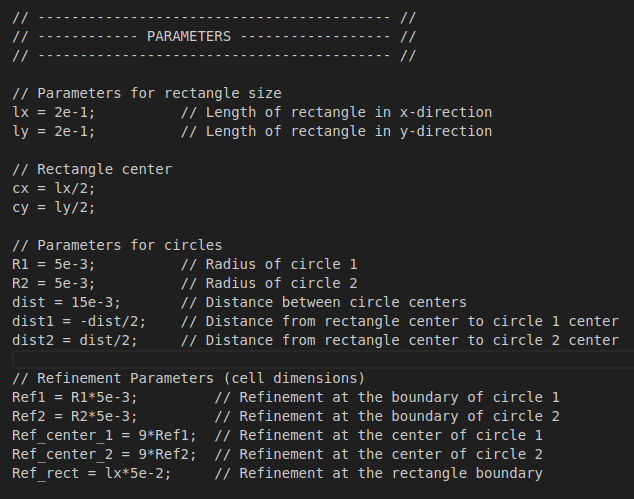
\includegraphics[width=0.7\textwidth]{Images/Gmsh_parameters.png}
    \end{center}
\end{frame}

\begin{frame}{Implementation: mesh generation II}
    The mesh sets different tags to the different regions of the domain, the tags are:
    \begin{center}
        \begin{tabular}{|c|l|}
            \hline
            Tag & Region \\
            \hline
            1 & Domain \\
            2 & Boundary of the domain \\
            11 & Conductor 1 \\
            12 & Conductor 2 \\
            \hline
        \end{tabular}
    \end{center}
    The mesh is then exported in \texttt{.m} format, a Matlab/Octave struct that contains all the mesh elements, saved in the file \texttt{mesh\_two\_circ\_cond.m}. This file is then read by the Octave code.
\end{frame}

\begin{frame}{Implementation: mesh generation III}
    Left: the full mesh; Right: the mesh around the conductors.
    \begin{center}
        \begin{minipage}{0.48\textwidth}
            \centering
            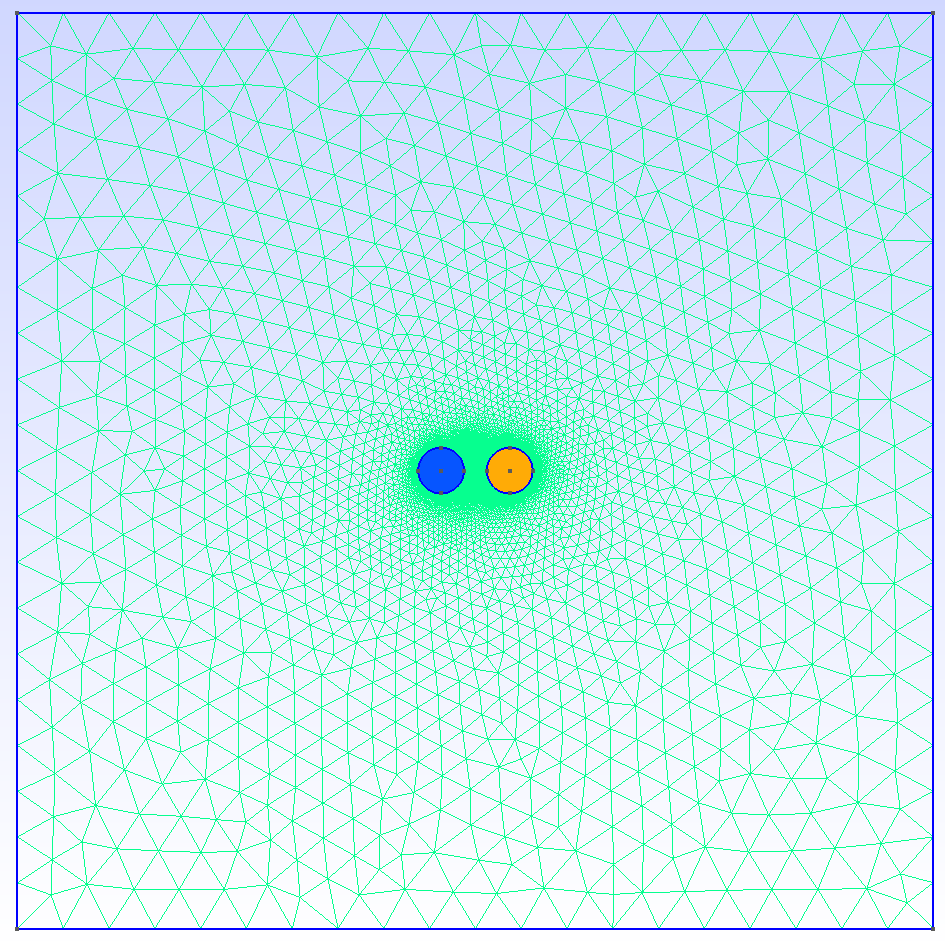
\includegraphics[width=\textwidth]{Images/Mesh_full.png}
        \end{minipage}\hfill
        \begin{minipage}{0.48\textwidth}
            \centering
            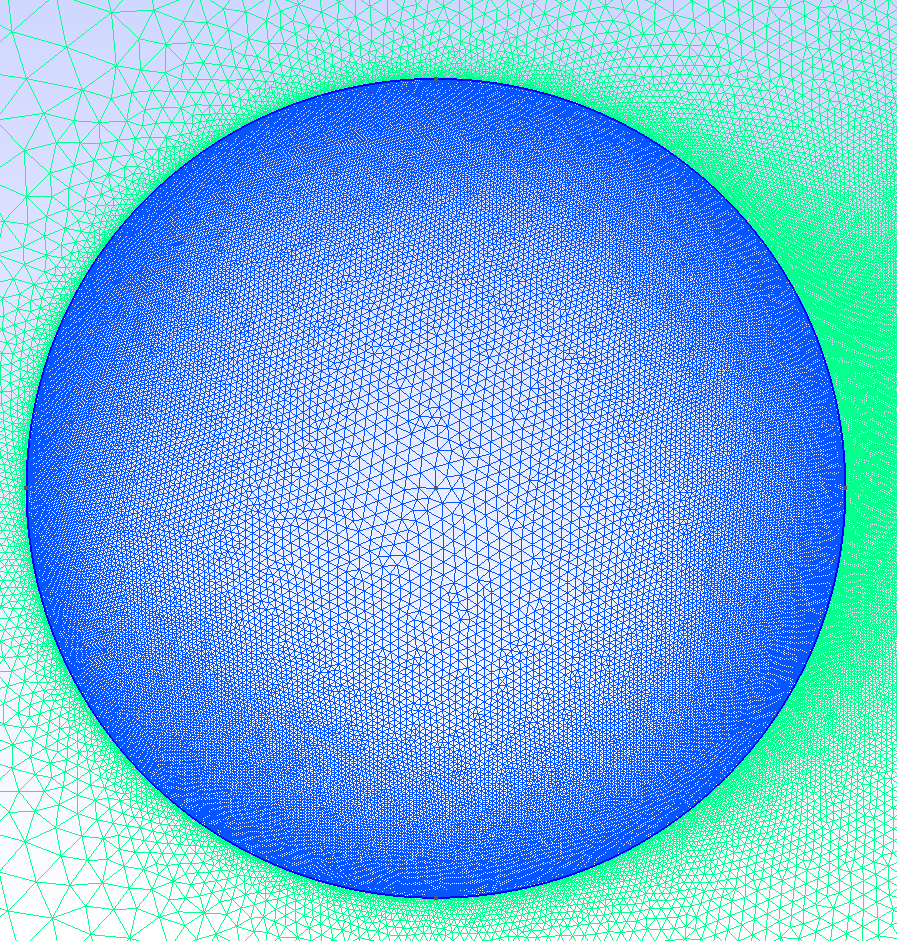
\includegraphics[width=\textwidth]{Images/Mesh_cond.png}
        \end{minipage}
    \end{center}
\end{frame}

\subsection{Main function}
\begin{frame}{Implementation: Main function (Description)}
    The function \texttt{FEM\_two\_conductors\_AC.m} implements the FEM method as described for 2 conductors. The main steps of the function are:
    \begin{enumerate}
        \item Load the necessary libraries (\texttt{msh}, \texttt{fpl}, \texttt{bim}).
        \item Load the mesh and saves the data to a struct (called \texttt{m}) and compute for each element area and gradient of basis functions.
        \item Extract the cells relative to the conductors and the boundary, compute $\mu$ and $\sigma$ with the correct node data.
        \item Assemble the Matrices $\frac{1}{\mu}S$, $j \omega \sigma M$, $j \omega \sigma Q$ and $j \omega \sigma W$, the full block system matrix and the block rhs vector.
        \item Solve the linear system applying homogeneous Dirichlet boundary conditions to obtain the total magnetic vector potential $A$ and the source magnetic vector potential $A_s$. Output the results in the specified format.
    \end{enumerate} 
\end{frame}

\begin{frame}[fragile]{1. FEM\_two\_conductors\_AC: Signature and Setup}
\small
\begin{lstlisting}
function [A, Js] = FEM_two_conductors_AC( mesh_file_name, freq, I_1, I_2, ...
                    mu_0, mu_r_1, mu_r_2, sigma_C_1, sigma_C_2, output_type)
  % Solve the eddy-current problem for two conductors at a given frequency.
  %
  % Inputs:
  %   mesh_file_name    : path to a .m mesh file generated by Gmsh
  %   freq              : excitation frequency [Hz]
  %   I_1, I_2          : total currents in conductors 1 and 2 [A]
  %   mu_0              : vacuum permeability
  %   mu_r_1, mu_r_2    : relative permeabilities of conductors
  %   sigma_C_1, sigma_C_2 : conductivities of conductors [S/m]
  %   output_type       : can be 'paraview' (results are written to .vtu files),
  %                       'octave' (results are plotted in Octave),
  %                       or 'off' (no output is produced)
  %
  % Outputs:
  %   A               : nodal values of magnetic vector potential A 
  %   Js              : source current density in each conductor

  pkg load msh fpl bim

\end{lstlisting}
\end{frame}

\begin{frame}[fragile]{2. FEM\_two\_conductors\_AC: Mesh Loading \& Preprocessing}
\scriptsize
\begin{lstlisting}[firstnumber=22]
  ## MESH PARAMETERS
  %--- Define region identifiers in the Gmsh .m file
  cell_id.external = 1;     % outer domain tag
  cell_id.bc  = 2;          % outer boundary tag
  cell_id.conduct_1 = 11;   % first conductor tag
  cell_id.conduct_2 = 22;   % second conductor tag


  ## MESH LOADING
  disp('Loading data ...')
  source (mesh_file_name);

  %--- Build octave mesh structure 'm'
  m.p = msh.POS'([1 2], :); % mesh nodes coordinates as 2xN
  x = msh.POS(:, 1);        % x-coordinates
  y = msh.POS(:, 2);        % y-coordinates
  m.e = msh.LINES';         % mesh edges
  % (reformat Gmsh linedata to match bim format)
  m.e(5, :) = m.e(3, :); m.e(3, :) = 0; m.e(7, :) = 1;
  m.t = msh.TRIANGLES';     % mesh elements (mesh triangles)

  %--- compute area of each element (m.area), and gradient of basis functions (m.shg)
  m = bim2c_mesh_properties (m);
  
\end{lstlisting}
\end{frame}

\begin{frame}[fragile]{3. FEM\_two\_conductors\_AC: Extracting Submeshes \& Node Data}
\scriptsize
\begin{lstlisting}[firstnumber=47]
  ## EXTRACT CONDUCTORS AND BOUNDARY NODES
  % conduct_1_nodes, conduct_2_nodes, bc_nodes are vectors containing respectively
  % the indices of the nodes in 1st conductor, 2nd conductor, external boundary
  [~, conduct_1_nodes, ~] = msh2m_submesh (m, [], cell_id.conduct_1);
  [~, conduct_2_nodes, ~] = msh2m_submesh (m, [], cell_id.conduct_2);
  bc_nodes = bim2c_unknowns_on_side (m, cell_id.bc);


  ## SETTING PARAMETERS
  omega = 2*pi*freq;  % angular frequency, is a scalar

  %--- Build nodal mu vector: mu0 in external region, mu_0*mu_r in conductors
  mu = ones(columns(m.p), 1) * mu_0;
  mu(conduct_1_nodes) = mu(conduct_1_nodes) * mu_r_1;
  mu(conduct_2_nodes) = mu(conduct_2_nodes) * mu_r_2;

  %--- Build nodal sigma vector: 0 in external region, sigma_C in conductors
  sigma = zeros(columns(m.p), 1);
  sigma(conduct_1_nodes) = sigma_C_1;
  sigma(conduct_2_nodes) = sigma_C_2;
  
\end{lstlisting}
\end{frame}

\begin{frame}[fragile]{4. FEM\_two\_conductors\_AC: Assembly of Linear System}
\scriptsize
\begin{lstlisting}[firstnumber=69]
  ## ASSEMBPLING SYSTEM
  disp('Assembling system ...')

  S = bim2a_laplacian(m, 1, 1./mu);           % Laplacian matrix with mu as coefficient

  M = reaction_full(m, 1, omega.*sigma.*i);   % Full mass matrix with sigma as coefficient

  f = bim2a_rhs(m, 1, 1);                     % Right-hand side vector

  q_1 = zeros(columns(m.p), 1);
  q_1(conduct_1_nodes) = f(conduct_1_nodes);  % conductor 1 specific source vector

  q_2 = zeros(columns(m.p), 1);
  q_2(conduct_2_nodes) = f(conduct_2_nodes);  % conductor 2 specific source vector

  Q = [omega.*sigma.*i.*q_1, omega.*sigma.*i.*q_2]; % om * sigma * j * Q

  W = [omega*sigma_C_1*i*sum(q_1), 0; 0, omega*sigma_C_2*i*sum(q_2)]; % om * sigma * j * W

  %--- Assemble global system
  System = [S+M, Q; Q.', W];
  Rhs = [zeros(columns(m.p), 1); -I_1; -I_2];
  
\end{lstlisting}
\end{frame}

\begin{frame}[fragile]{5. FEM\_two\_conductors\_AC: Solve Linear System and Postprocessing}
\scriptsize
\begin{lstlisting}[firstnumber=93]
  ## SOLVE LINEAR SYSTEM
  disp('Solving system ...')

  % Internal nodes are all nodes except the boundary nodes, with the addition of 
  % the two unknowns for the source magnetic vector potential in the conductors
  internal_nodes = setdiff (1:numel(x)+2, bc_nodes);
  A_J = zeros(columns(m.p)+2, 1);   % setup solution vector

  % solve linear system applying omogeneous Dirichlet boundary conditions
  A_J(internal_nodes) = System(internal_nodes, internal_nodes) \ Rhs(internal_nodes);

  ## GET RESULTS
  %--- Split solution into A (first N) and As (last 2)
  A = A_J(1:end-2);
  Js = [ -omega*sigma_C_1*j*A_J(end-1); -omega*sigma_C_2*j*A_J(end)];

  %--- Compute current density J = -omega*sigma*i*A
  J = -omega.*sigma.*i.*A;
  J(conduct_1_nodes) += Js(1);
  J(conduct_2_nodes) += Js(2);
  
\end{lstlisting}

\begin{lstlisting}[firstnumber=115]
  ## OUTPUT RESULTS
  if strcmp(output_type, "paraview") % Output results to paraview using fpl functions ...

\end{lstlisting}

\begin{lstlisting}[firstnumber=137]
  elseif strcmp(output_type, "octave")  % Plot results using patch function of octave ...

\end{lstlisting}
\end{frame}

\subsection{bim2c\_mesh\_properties}
\begin{frame}{bim2c\_mesh\_properties (Description)}
    The mesh properties (area and shape functions gradients) are computed with the call to the function \texttt{bim2c\_mesh\_properties} of the \texttt{bim} package. This functions calls other subfunctions, one to compute the area of each triangle, and another to compute the gradients of the shape functions.
    The variables used in the subfunctions are:
    \begin{itemize}
        \item \texttt{p}: Matrix containing the coordinates of the mesh nodes (2xN).
        \item \texttt{e}: Matrix containing the edges of the boundary of the mesh (actually it is not used in this context)
        \item \texttt{t}: Matrix containing the triangles of the mesh (4xNT element connectivity + tags).
    \end{itemize}
    The results are saved in the mesh struct \texttt{m} under \texttt{m.area}, \texttt{m.wjacdet} and \texttt{m.shg}. The field \texttt{wjacdet} contains the weighted Jacobian determinants for each node in each element.
\end{frame}

\begin{frame}{bim2c\_mesh\_properties: Element Area I}
\small
Let each triangle have nodes with coordinates $((x_1,y_1), (x_2,y_2), (x_3,y_3))$.
\textbf{Jacobian matrix} for the affine map:
\[
    J \;=\;
    \begin{pmatrix}
        x_2 - x_1 & x_3 - x_1 \\[3pt]
        y_2 - y_1 & y_3 - y_1
    \end{pmatrix},
    \quad
    \det J \;=\;(x_2 - x_1)(y_3 - y_1)\;-\;(x_3 - x_1)(y_2 - y_1)
\]

\textbf{Element area}:
\[
    A_K \;=\;\tfrac12\,|\det J|
    \quad\Longrightarrow\quad
    A_K = \tfrac12\,\bigl|(x_2-x_1)(y_3-y_1)-(x_3-x_1)(y_2-y_1)\bigr|
\]
\textbf{In the code}:
\begin{itemize}
    \item weight: 1x3 node weights for reference triangle: $\mathtt{weight[i]} = \tfrac13$ 
    \item jacdet: 1xNT Jacobian determinants for each triangle
    \item wjacdet: 3xNT weighted Jacobian determinants for each node in each triangle: $\mathtt{wjacdet[i][e]} = \tfrac12 * \mathtt{weight[i]} * \mathtt{jacdet[e]}$ 
    \item area: NTx1 element areas: $\mathtt{area[e]} = \sum_{i=1}^{3} \tfrac12 * \mathtt{weight[i]} * \mathtt{jacdet[e]}$
\end{itemize}
\end{frame}

\begin{frame}[fragile]{bim2c\_mesh\_properties: Element Area II}
\scriptsize
\begin{lstlisting}[firstnumber=374]
function [b] = computearea(p,e,t,string)

  % p: 2xN node coords, t: 4xNT element connectivity + tags
  weight      = [1/3, 1/3, 1/3];    % equal weights for 3 nodes
  areakk      = 1/2;                % factor 1/2 in area formula
  Nelements   = columns(t);         % number of triangles
  
  % Build Jacobian entries for each element K
  jac([1,2],:) = [ p(1,t(2,:)) - p(1,t(1,:)); p(1,t(3,:)) - p(1,t(1,:)) ];
  jac([3,4],:) = [ p(2,t(2,:)) - p(2,t(1,:)); p(2,t(3,:)) - p(2,t(1,:)) ];
  % determinant of Jacobian
  jacdet = jac(1,:) .* jac(4,:) - jac(2,:) .* jac(3,:);   
  
  % ... Error handling ...
  
  % Weighted jacobian for each local node i
  for inode = 1:3
    wjacdet(inode,:) = areakk .* jacdet .* weight(inode);
  endfor
  
  % Return weighted jacobian or area
  if string == "wjac"
    b = wjacdet;                  % 3xNT array of 1/2*det*1/3
  elseif string == "area"
    b = sum(wjacdet)';            % NTx1 vector of element areas
  endif

endfunction
\end{lstlisting}
\end{frame}

\begin{frame}{bim2c\_mesh\_properties: Gradient of shape functions I}
\small
Let each triangle have nodes with coordinates $((x_1,y_1), (x_2,y_2), (x_3,y_3))$.
\textbf{Gradient of linear “hat” basis} \(\varphi_i\) on each triangle:
\begin{align*}
    \nabla\varphi_1 = \frac{1}{2A_K}
        \begin{pmatrix} y_2 - y_3 \\[3pt] -(x_2 - x_3) \end{pmatrix},
    \\
    \nabla\varphi_2 = \frac{1}{2A_K}
        \begin{pmatrix} y_3 - y_1 \\[3pt] -(x_3 - x_1) \end{pmatrix},
    \\
    \nabla\varphi_3 = \frac{1}{2A_K}
        \begin{pmatrix} y_1 - y_2 \\[3pt] -(x_1 - x_2) \end{pmatrix}.
\end{align*}
Note that on each triangle the gradients are constant, and the area $A_K$ is computed as in the previous slide. \\
In code for each element 'e' these are assembled into a 2x3 array 'shg(:,:,e)'.
\end{frame}

\begin{frame}[fragile]{bim2c\_mesh\_properties: Gradient of shape functions II}
\scriptsize
\begin{lstlisting}[firstnumber=427]
function [shg] = shapegrad(p,t)
  
  ## Compute  the gradient of the hat functions
  
  x0 = p(1,t(1,:));
  y0 = p(2,t(1,:));
  x1 = p(1,t(2,:));
  y1 = p(2,t(2,:));
  x2 = p(1,t(3,:));
  y2 = p(2,t(3,:));

  denom = (-(x1.*y0) + x2.*y0 + x0.*y1 - x2.*y1 - x0.*y2 + x1.*y2);
  shg(1,1,:)  =  (y1 - y2)./denom;
  shg(2,1,:)  = -(x1 - x2)./denom;
  shg(1,2,:)  = -(y0 - y2)./denom;
  shg(2,2,:)  =  (x0 - x2)./denom;
  shg(1,3,:)  =  (y0 - y1)./denom;
  shg(2,3,:)  = -(x0 - x1)./denom;

endfunction
\end{lstlisting}
\end{frame}

\subsection{Matrices and RHS}
\begin{frame}[fragile]{Matrices and RHS: Assembly Algorithm}
\scriptsize
\begin{block}{Pseudocode Classic FEM}
\begin{verbatim}
for K = 1:Nelements
  Compute local element matrix Mloc_K 3x3
  for i = 1:3
    for j = 1:3
      Scatter into global: A(I,J) = A(I,J) + Mloc_K(i,j);
    endfor
  endfor
endfor
\end{verbatim}
\end{block}

For performace reasons, in this code the assembly of all the matrices and RHS is done in a vectorized way, with the following structure:
\begin{block}{Pseudocode Octave Vectorized Assembly}
\begin{verbatim}
Mloc = zeros(3,3,Nelements);
for i = 1:3
  for j = 1:3
    Compute Mloc(i,j,:) in parallel over all elements
  endfor
endfor
Single sparse call builds the global matrix
\end{verbatim}
\end{block}
\end{frame}

\begin{frame}{Laplacian matrix (Description)}
    The Laplacian matrix is computed in \texttt{bim2a\_laplacian}. \\
    Local assembly:
    \begin{align*}
        [L^{t}]_{ij} &= \int_{t} \frac{1}{\mu} \nabla \phi_i \cdot \nabla \phi_j \, ds = \frac{1}{\mu_t} \nabla \phi_{t,i} \cdot \nabla \phi_{t,j} \, Area_t
    \end{align*}
    \texttt{bim2a\_laplacian} has the following inputs:
    \begin{itemize}
        \item \texttt{mesh}: mesh struct.
        \item \texttt{epsilon}: vector of element data (1xNT).
        \item \texttt{kappa}: vector of node data (1xN).
    \end{itemize}

\end{frame}

\begin{frame}[fragile]{bim2a\_laplacian (Code)}
\scriptsize
\begin{lstlisting}[firstnumber=41]
function A = bim2a_laplacian (mesh, epsilon, kappa)
  % ... Check input ...
  p      = mesh.p;  % 2xN matrix of node coordinates
  t      = mesh.t;  % 4xNT matrix of element connectivity + tags
  nnodes = columns(p); % number of nodes
  nelem  = columns(t); % number of elements
  % ... Turn scalar input to a vector of appropriate size ...

  Lloc = zeros(3, 3, nelem); % 3x3 matrix for each triangle in the mesh

  ## To integrate constants over each triangle we need to multiply by
  ## the triangle area. Multiply by the diffusion coefficient now tu
  ## simplify subsequent computations. Use inverse average for the
  ## diffusion coefficient.
  kappaepsilonareak = reshape (3./sum (1./kappa(:)(mesh.t (1:3)), 1)(:) .* epsilon(:) .* mesh.area(:), 1, 1, nelem);
  shg = mesh.shg(:,:,:);  % 2x3xNT matrix of gradients of shape functions
  
  ## Computation
  for inode = 1:3
    for jnode = 1:3
      ginode(inode,jnode,:) = mesh.t(inode,:); % global node indices
      gjnode(inode,jnode,:) = mesh.t(jnode,:);
      Lloc(inode,jnode,:)   = sum (shg(:,inode,:) .* shg(:,jnode,:), 1) .* kappaepsilonareak;
    endfor
  endfor

  ## Assemble the local (full) matrices into one global (sparse) matrix
  A = sparse (ginode(:), gjnode(:), Lloc(:));

endfunction
\end{lstlisting}
\end{frame}

\begin{frame}{Mass matrix (Description)}
    The mass matrix is computed in \texttt{reaction\_full}. \\
    Local assembly:
    \begin{align*}
        [B^{t}]_{ij}
        = \int_{t} \delta_{t}\,\varphi_i\,\varphi_j \,dA
        = \delta_{t}\,det(J_t)\,\int_{\hat{t}} \hat{\varphi}_i\,\hat{\varphi}_j \,d\hat{A} = \\
        = \delta_{t}\,2\,\mathrm{Area}_{t}\,\frac{1}{24}
          \begin{pmatrix}2&1&1\\1&2&1\\1&1&2\end{pmatrix}_{ij}
    \end{align*}
    where $\hat{t}$ is the reference triangle and $\hat{\varphi}_i$ are the reference basis functions. \\
    \texttt{reaction\_full} has the following inputs:
    \begin{itemize}
        \item \texttt{mesh}: mesh struct.
        \item \texttt{delta}: vector of element data (1xNT).
        \item \texttt{zeta}: vector of node data (1xN).
    \end{itemize}
\end{frame}

\begin{frame}[fragile]{reaction\_full (Code)}
\scriptsize
\begin{lstlisting}[language=Octave,firstnumber=19]
function C = reaction_full(mesh, delta, zeta)
  % ... Check input ...
  p      = mesh.p;    % 2xN node coords
  t      = mesh.t;    % 4xNT connectivity + tags
  nnodes = columns(p);
  nelem  = columns(t);
  % ... Turn scalar input to a vector of appropriate size ...

  % Local element matrices: one 3x3 block per triangle
  Blocmat = zeros(3,3,nelem);
  phi_ij  = [2 1 1; 1 2 1; 1 1 2] / 24;

  % Build each local block in vectorized loops
  for inode = 1:3
    for jnode = 1:3
      ginode(inode,jnode,:) = mesh.t(inode,:);   % global rows
      gjnode(inode,jnode,:) = mesh.t(jnode,:);   % global cols
      Blocmat(inode,jnode,:) = ...
        phi_ij(inode,jnode) .* 2 .* mesh.area(:) .* delta(:);
    endfor
  endfor

  % Assemble sparse element-wise matrix and apply zeta
  C0 = sparse(ginode(:), gjnode(:), Blocmat(:));
  C  = C0 * sparse(diag(zeta));
endfunction
\end{lstlisting}
\end{frame}

\begin{frame}{RHS vector (Description)}
    The load vector is computed in \texttt{bim2a\_rhs}. \\
    Local assembly on triangle \(t\):
    \[
      [b^{t}]_{i}
      = \int_{t} f_{t}\,g(x)\,\varphi_i(x)\,dA
      \;\approx\;
      f_{t}\,g(x_{i})\,\frac{\mathrm{Area}_{t}}{3}
      \;=\;
      f_{t}\,g_{i}^{t}\,\texttt{wjacdet}_{i,t}
    \]
    where \(\texttt{wjacdet}_{i,t}=\tfrac12\det(J_t)\times\tfrac13\).  
    \bigskip

    \texttt{bim2a\_rhs} has the following inputs:
    \begin{itemize}
      \item \texttt{mesh}: mesh struct, with \texttt{wjacdet} precomputed.
      \item \texttt{f}: element-wise source term (1xNT).
      \item \texttt{g}: nodal coefficient (1xN).
    \end{itemize}
\end{frame}

\begin{frame}[fragile]{bim2a\_rhs (Code)}
\scriptsize
\begin{lstlisting}[language=Octave,firstnumber=40]
function b = bim2a_rhs(mesh, f, g)
  % ... input checks ...
  nnodes = columns(mesh.p);
  nelem  = columns(mesh.t);
  % ... Turn scalar input to a vector of appropriate size ...

  % Extract g at each triangle's nodes
  g = g(mesh.t(1:3,:));        % 3xNT matrix
  wjacdet = mesh.wjacdet;      % 3xNT weighted jacobian

  % Build local contributions: Blocmat(i,K) = f_K * g_i^K * wjacdet(i,K)
  Blocmat = zeros(3, nelem);
  for inode = 1:3
    Blocmat(inode,:) = f.' .* g(inode,:) .* wjacdet(inode,:);
  endfor

  % Global node indices for each local position
  gnode = mesh.t(1:3,:);       % 3xNT

  % Assemble sparse right-hand side vector
  b = sparse(gnode(:), 1, Blocmat(:));
endfunction
\end{lstlisting}
\end{frame}


\section{Results}
\begin{frame}{Simulation Results}

\end{frame}

\section{Conclusion}
\begin{frame}{Conclusion}
    \begin{itemize}
        \item Summary of findings
        \item Future work
    \end{itemize}
\end{frame}

% References
\begin{frame}{References}
    % \footnotesize
    % \begin{thebibliography}{99}
        % \bibitem{sadiku} M. N. O. Sadiku, \emph{Numerical Techniques in Electromagnetics}, CRC Press, 2000.
        % \bibitem{taflove} A. Taflove, S. C. Hagness, \emph{Computational Electrodynamics: The Finite-Difference Time-Domain Method}, Artech House, 2005.
    % \end{thebibliography}
\end{frame}

\end{document}